% clase 2016/02/15

\chapter{Ecuaciones de segundo orden. Series de Fourier}
\label{chap:EcuacionesSegundoOrden}

\section{Método de separación de variables}\index{Ecuación! del calor}

	Al empezar el curso ya vimos un ejemplo: la ecuación del calor en una dimensión con datos de contorno Dirichlet homogéneos.\index{Método!separación de variables}

	\begin{example}{1. Ecuación del calor con contorno Dirichlet}
		\[
		\begin{cases}
		u_t - u_{xx} = 0 & x \in (0,L), \quad t > 0 \\
		u(0,t) = u(L,t) = 0 & t > 0 \\
		u(x,0) = f(0) & x \in [0,L]
		\end{cases}
		\]

		La ecuación del medio es el dato de contorno de Dirichlet\index{Condición! de contorno Dirichlet} homogéneo, es decir, que especifica el dato en los extremos.

		Llegamos con separación de variables a que la solución del problema podía ser escrita como:

		\[ u(x,t) \eqexpl{?} \sum^{\infty}_{k=1} a_k e^{-(\frac{k\pi}{L})^2 t} \sin \left( \frac{k\pi}{L} x \right) \]
		donde
		\[ f(x) \eqexpl{?} \sum^{\infty}_{k=1} a_k \sin \left( \frac{k\pi}{L}x \right) \]
	\end{example}


	\begin{example}{2. Ecuación de calor con contorno de Neumann\index{Condición! de contorno Neumann}}

		\[
		\begin{cases}
		u_t - u_{xx} = 0 & x \in (0,L), t > 0 \\
		u_x(0,t) = u_x(L,t) = 0 \\
		u(x,0) = f(x) \in [0,L]
		\end{cases}
		\]

		Esta condición indica que no hay flujo de calor entre la varilla y cualquier punto fuera, incluidos los extremos. Esperamos que al final, cuando el tiempo tienda a infinito el calor se haya distribuido a lo largo de la varilla y la temperatura sea constante a lo largo de esta. El valor de esto probablemente sea el promedio.

		\begin{figure}[thbp]
		\centering
		\inputtikz{transmisionCalorNeumann}
		\caption{}
		\label{fig:transmisionCalorNeumann}
		\end{figure}

		Empecemos con el método de separación de variables. Buscamos $u(x,t) = X(t) \cdot T(t)$ que sea solución de la ecuación con el contorno (el dato inicial se tratará después).


		\[
		\begin{array}{l}
			0 = u_t - u_{xx} = T' X - T X'' \\
			0 = u_x (0,t) = T(t) X'(0) \\
			0 = u_x (L,t) = T(t) X'(L)
		\end{array}
		\]

		De lo que obtenemos:

		\[ \frac{T'(t)}{T(t)} = \frac{X''(x)}{X(x)} \quad \forall x, \forall t \]

		Como estamos igualando dos cocientes de funciones de variables diferentes que es cierto $\forall x, \forall t$, esto solo puede significar que ambos cocientes son constantes. A esta proporción la llamaremos $\lambda$:

		\[ \frac{T'}{T} = \frac{X''}{X} = \lambda \in \mathbb{R} \]

		% Método general? SI
		Resolvemos la EDO en X:

		\[
		\left\{ \begin{array}{l}
		X'' = \lambda X \\
		X'(0) = X'(L) = 0
		\end{array} \right. \quad\quad \text{(problema de contorno)}
		\]

		Veamos carios casos en función de $\lambda$:

		\begin{itemize}
			\item $\lambda = 0$

				Cuando $\lambda = 0 \Rightarrow X'' = 0$. Así que tenemos que $X'$ tiene que ser constante y $X$ lineal. Pero además los datos iniciales nos indican el valor de $X'$, al ser constante.

				\[ \left.
				\begin{array}{l}
					X(x) = a + bx \\
					\left.
					\begin{array}{r}
						X'(x) = b \\
						X'(0) = X'(L) = 0
					\end{array} \right\} \Rightarrow b = 0
				\end{array} \right\} \Rightarrow X \equiv a \]

				Tiene una solución no trivial que es $\lambda = 0, X=a_0$.

			\item $\lambda > 0$ con $\lambda = \mu^2$, $\mu \in \mathbb{R}$

				Lo cual nos lleva a una EDO de orden 2, que se resolvería con el polinomio característico.

				\[ \text{Las soluciones siguen } \left\{
				   \begin{array}{l}
				   	X(x) = a \cdot e^{\mu x} + b \cdot e^{-\mu x} \\
				   	X'(x) = \mu (a\cdot e^{\mu x} - b\cdot e^{-\mu x})
				   \end{array} \right.
				\]

				\[ \left. \begin{array}{l}
					0 = X'(0) \Rightarrow \mu(a - b) = 0 \\
					0 = X'(L) \Rightarrow \mu(a \cdot e^{\mu L} - b \cdot e^{-\mu L}) = 0
				\end{array} \right\}
					\Rightarrow … \Rightarrow a = b = 0
				\]


			\item $\lambda < 0$ con $\lambda = - \mu^2$

				Aquí volvemos a emplear el polinomio característico pero llegaremos a soluciones complejas.

			 	\[ \text{Solución} \left\{
				   \begin{array}{l}
				   	X(x) = a \cos(\mu x ) + b \sin( \mu x) \\
				   	X'(x) = -a \mu \sin(\mu x) + b \mu \cos(\mu x)
				   \end{array} \right.
				\]

			 	\[
			 		\begin{array}{l}
			 		0 = X'(0) = b \mu \\
			 		0 = X'(L)
			 		\end{array} \Rightarrow b = 0 \Rightarrow \left\{ \begin{array}{l}
			 			X(x) = + a \cos (\mu x ) \\
			 			X'(x) = -a \mu \sin (\mu x)
			 		\end{array} \right.
			 	\]

			 	De lo que obtenemos que

			 	\[0 = X'(L) = -a \mu \sin(\mu L) \Rightarrow \mu L = k \pi , \quad k = 1,2,…\]



		\end{itemize}

		Conclusión:
				\begin{align*}
					\lambda_0 = 0\quad & \quad X_0 = a_0 \\
					\lambda_k = - \left(\frac{k\pi}{L}\right)^2\quad & \quad X_k(x) = a_k \cos (\frac{k \pi}{L}x)
				\end{align*}

			 	EDO para T (para las $\lambda$ encontradas antes)

			 	\[\lambda_0 = 0 \Rightarrow T'_0 \equiv 0 \Rightarrow T_0 \equiv \alpha_0\]
			 	\[\lambda_k = - \left(\frac{k\pi}{L}\right)^2 \Rightarrow T'_k = -\left(\frac{k\pi}{L}\right)^2 T_k \Rightarrow T_k (t) = \alpha_k e^{-\left(\frac{k\pi}{L}\right)^2 t} \]

			 	Soluciones particulares:
			 	\[u_0(x,t) = A_0, \quad u_k (x,t) = A_k e^{-\left(\frac{k \pi}{L} \right)^2 t} \cos \left( \left( \frac{k \pi}{L}\right) x \right) \]

			 	Dato inicial: $u(x,0) = f(x)$

			 	Idea: $u(x,t) \eqexpl{?} A_0 + \sum\limits_{k=1}^{\infty} A_k e^{- \left( \frac{k \pi}{L} \right)^2 t}  \cos \left( \frac{k \pi}{L} x \right)$

			 	Pero claro, no sabemos calcular $A_k$. ¿O como calculamos la convergencia? ¿Cómo calculamos las derivadas?


		\end{example}

		\begin{example}{3: Cuerda vibrante}

			Veamos una cuerda de guitarra en tensión. La guitarra está atada en los extremos y la altura sobre el eje horizontal es $u$.

			\begin{figure}[thbp]
			\centering
			\inputtikz{cuerdaGuitarra}
			\caption{}
			\label{fig:cuerdaGuitarra}
			\end{figure}


			\[  \begin{cases}
				u_{tt} - u_{xx} = 0 \quad \text{ 2º orden \quad 2 datos } \\
				u(0,t) = u(L,t) = 0 \quad \text{Dirichlet}\\
				u(x,0) = f(x) \\
				u_t(x,0) = g(x)
				\end{cases}
			\]

			Por separación de variables. Buscamos un $u(x,t) = X(t) T(t)$, solución de la ecuación con el contorno:
			\[ 0 = u_{tt} - u_{xx} = T'' X - T X''\]
			\[ \frac{T''}{T} = \frac{X''}{X} = \lambda \in \mathbb{R}\]

			EDO para $X$:

			\[\begin{cases}
				X'' = \lambda X \\
				X(0) = X(L) = 0
			\end{cases}
			\]

			Vemos que ha cambiado respecto al sistema anterior en que la última ecuación ya no relaciona las derivadas de $X$ sino $X$. De nuevo, buscamos las soluciones en función del valor de $\lambda$:

			\begin{itemize}
				\item $\lambda = 0$

					\[
					\left\{
					\begin{array}{l}
					X(x) = a + bx \\
					X(0) = 0 = X(L)
					\end{array}
					\right.
					\Rightarrow
					a = 0 = b
					\]

				\item $\lambda > 0$ con $\lambda = \mu^2$

					\[
					\left\{
					\begin{array}{l}
					X(x) = a \cdot e^{\mu x} + b \cdot e^{-\mu x} \\
					X(0) = 0 = X(L)
					\end{array}
					\right.
					\Rightarrow … \Rightarrow
					a = b = 0
					\]

				\item $\lambda < 0$ con $\lambda = -\mu^2$

					\[
					\left\{
					\begin{array}{l}
					X(x) = a\cos(\mu x) + b\sin(\mu x) \\
					X(0) = 0 = X(L)
					\end{array}
					\right.
					\Rightarrow X(0) = a \Rightarrow X(x) = b \sin(\mu x)
					\]

					\[ \Rightarrow X(L) = 0 = b \sin (\mu L) \Rightarrow \mu = \frac{k \pi}{L}\]

			\end{itemize}

			Con lo que llegamos a las soluciones no triviales:

			\[\lambda_k = - (\frac{k\pi}{L})^2, \quad X_k(x) = b_k \sin \left(\frac{k\pi}{L} \right) x\]


			Una vez que resolvemos la EDO para $X$, la resolvemos para $T$:

			\[T'' = \lambda T\]

			Es similar a la X así que tenemos:

			\[T''_k = - (\frac{k\pi}{L})^2 T_k \Rightarrow T_k (t) = \alpha_k \cos\left( \frac{k \pi}{L} t \right) + \beta_k \sin \left( \frac{k \pi}{L}t \right)\]

			Con lo que llegamos a las soluciones particulares:

			\[u_k(x,t) = A_k \cos \left(\frac{k\pi}{L} t\right) \sin \left(\frac{k\pi}{L}x\right) + B_k \sin \left(\frac{k\pi}{L}t\right)  \sin \left(\frac{k\pi}{L}x\right) \]

			Idea: Buscar

			\[u(x,t) \eqexpl{?} \sum_{k=1}^{\infty} A_k \cos \left(\frac{k\pi}{L} t\right) \sin \left(\frac{k\pi}{L} x  \right)+ B_k \sin \left(\frac{k\pi}{L}t \right) \sin \left(\frac{k\pi}{L}  x \right)\]

			Datos iniciales:
			\[ f(x) = u(x,0) \eqexpl{?} \sum^{\infty}_{k=1} A_k \sin \left(\frac{k\pi}{L} x  \right)\]

			Suponiendo que derivada e integral conmutan:

			\[ u_t (x,t) \eqexpl{?} \sum_{k} - A_k \left(\frac{k\pi}{L} \right) \sin \left(\frac{k\pi}{L}t \right) \sin \left(\frac{k\pi}{L}x \right) + B_k \left(\frac{k\pi}{L} \right) \cos \left(\frac{k\pi}{L}t \right) \sin \left(\frac{k\pi}{L}x \right)
			\]

			\[g(x) = u_t(x,0) \eqexpl{?} \sum_k B_k  \left(\frac{k\pi}{L} \right) \sin \left(\frac{k\pi}{L}x \right)\]

		\end{example}

		% clase 2016/02/16

		\begin{example}{4: Ondas con condiciones periódicas}\index{Ecuación!de ondas}\label{ec:ondas}

			Estudiemos, por ejemplo, las olas en alta mar. No tenemos un contorno fijo como antes, así que vamos a buscar soluciones que sean periódicas en los extremos. En este caso tendremos dos condiciones, llamadas condiciones de periodicidad\index{Condición! de periodicidad}. Hemos puesto dos porque lo observamos en segundo orden:

			\[u(-L,t) = u(L,t), \forall t\]
			\[u_x(-L,t) = u_x(L,t), \forall t\]

			El problema nos queda así:

			\[  \begin{cases}
				u_{tt} - u_{xx} = 0 \quad x  \in (-L,L)\footnotemark, t>0\\
				u(-L,t) = u(L,t), \forall t\\
				u_x(-L,t) = u_x(L,t), \forall t
				u(x,0) = f(x) \\
				u_t(x,0) = g(x)
				\end{cases}
			\]
			\footnotetext{Para que las cuentas cuadren mejor}

			Aplicamos el método de separación de variables:
			\[ \frac{T''}{T} = \frac{X''}{X} = \lambda \in \mathbb{R}\]

			EDO para $X$:
			\[\left\{\begin{array}{l}
				X'' = \lambda X \quad x \in (-L,L) \\
				X(-L) = X(L) \\
				X'(-L) = X'(L)
			\end{array}
			\right. \]

			\begin{itemize}
				\item $\lambda = 0$
					\[\left\{\begin{array}{l}
						X = a+bx \\
						X'(x) = b \\
						X(-L) = X(L) \quad \Rightarrow a + b(-L) = a + bL \Leftrightarrow b = 0
					\end{array}
					\right. \]

					Si $b = 0$ entonces la $a$ será arbitraria. $\Rightarrow \lambda_0 = 0$, $ X_0 \equiv a \in \mathbb{R}$


				\item $\lambda > 0$ con $\lambda = \mu^2$

					\[\begin{cases}
						X(x) = a\cdot e^{\mu x} + b \cdot e^{-\mu x} \\
						X'(x) = a\mu \cdot e^{\mu x} - b \mu \cdot e^{-\mu x}
					\end{cases}
					\Rightarrow a = b = 0 \]


				\item $\lambda < 0$ con $\lambda = -\mu^2$

					\[ X (x) = a \cos (\mu x) + b \sin (\mu x) \]

					\[\text{2 caminos: }\left\{\begin{array}{l}
						\text{ pensar }\rightarrow \mu = \frac{2\pi}{L} \\
						\text{ hacer cuentas }\footnotemark\rightarrow \left\{ \begin{array}{l}
							X(-L) = X(L) \\
							X'(-L) = X'(L)
						\end{array} \right.
					\end{array}
					\right. \]\footnotetext{se dejan como ejercicio}
			\end{itemize}

			Ajustamos $\mu$ para que $X$ sea periódica con periodo $2L k \Rightarrow … \Rightarrow \mu = \frac{k \pi}{L}$. Donde $2L$ es la longitud del intervalo. Por lo que llegamos a las soluciones:

			\[
			\lambda_k = -\left(\frac{k\pi}{L}\right)^2\quad\quad X_k(x) = a_k \cos \left( \frac{k\pi}{L} x \right) + b_k \sin \left( \frac{k\pi}{L} x \right)
			\]

			EDO para $T$:

			\[ \lambda_0 = 0 \rightarrow T''=0 \rightarrow T(t) = \alpha_0 + \beta_0 t\]

			\[ \lambda_k = - \left( \frac{k\pi}{L} \right)^2, \quad T''_k = - \left( \frac{k\pi}{L} \right)^2 T_k \]

			\[\Rightarrow T_k(t) = \alpha_k \cos \left( \frac{k\pi}{L} t \right) + \beta_k \sin \left( \frac{k\pi}{L} t \right) \]

			Soluciones particulares de la EDO para T:

			\[u_k (x,t) = T_k(t) \cdot X_k(x) \quad k = 0,1,2,… \]


			Soluciones en forma de serie:

			\[u(x,t) = \sum_{k=1}^{\infty} u_k (x,t) \rightarrow \text{ Ajustar datos } f,g \]

			¿Converge esta serie?. La ecuación del calor era buena, ya que al tener una exponencial menor que 0 tendía a 0 muy rápido. En la ecuación de ondas la parte temporal no ayuda ya que tiene un comportamiento cualitativo distinto.

			Volvemos a nuestras soluciones particulares:

			\[u_0(x,t) = a_0 + b_0t\]

			% lo siento mucho si hay una errata en estas fórmula y te toca editarlas.

			\begin{align*}
			u_k(x,t) = &\left(\alpha_k \cos \left( \frac{k \pi}{L} t \right) + \beta_k \sin \left( \frac{k \pi}{L} t \right) \right) \\
			\cdot &\left(a_k \cos \left( \frac{k \pi}{L} x \right) + b_k \sin \left( \frac{k \pi}{L} x \right) \right)
			\end{align*}
			\begin{align*}
			u_k(x,t) = &\left(A_k \cos \left( \frac{k \pi}{L} x \right) + B_k \sin \left( \frac{k \pi}{L} x \right) \right) \cos \left( \frac{k \pi}{L} t \right)\\
			+ &\left(C_k \cos \left( \frac{k \pi}{L} x \right) + D_k \sin \left( \frac{k \pi}{L} x \right) \right) \sin \left( \frac{k \pi}{L} t \right)
			\end{align*}




			\[u_k(x,t) = T_k(t) X_k(t) \quad (k=0,1,2,…)\]


			y soluciones en forma de serie:

			\[ u(x,t) = u_0 + \sum_k u_k \]

			\begin{align*}
				u(x,t) = A_0 + C_0 t &+ \sum^{\infty}_{k=1} \left(A_k \cos \left( \frac{k \pi}{L} x \right) + B_k \sin \left( \frac{k \pi}{L} x \right) \right) \cos \left( \frac{k \pi}{L} t \right)\\
				&+ \sum^{\infty}_{k=1} \left(C_k \cos \left( \frac{k \pi}{L} x \right) + D_k \sin \left( \frac{k \pi}{L} x \right) \right) \sin \left( \frac{k \pi}{L} t \right)
			\end{align*}

			En $t = 0$

			\[f(x) = u(x,0) = A_0 + \sum_{k=1}^{\infty} A_k \cos \left( \frac{k \pi}{L} x \right) + B_k \sin \left( \frac{k \pi}{L} x \right) \]

			\[g(x) = u_t (x,0) = C_0 + \sum_{k=1}^{\infty} \left(\frac{k \pi}{L}\right) \left( C_k \cos \left( \frac{k \pi}{L} x \right) + D_k \sin \left( \frac{k \pi}{L} x \right)\right) \]


		\end{example}

		De 4 ejemplos hemos obtenido la misma solución:

		\[ f(x) = \sum_{k=1}^{\infty} b_k \sin \left( \frac{k \pi}{L} x \right), \quad x \in (0,L) \]

		\[ f(x) = a_0 + \sum^{\infty}_{k=1} a_k \cos \left( \frac{k \pi}{L} x \right), \quad x \in (0,L) \]

		\(
		f(x) \qeq a_0 + \sum^{\infty}_{k=1} a_k \cos \left( \frac{k \pi}{L} x \right) + b_k \sin \left( \frac{k \pi}{L} x \right), \quad x \in (-L,L)
		\)

		Ésta última es combinación de las dos anteriores, y nos lleva al problema que queremos resolver. ¿Es una solución?, y en ese caso: ¿Es única?.\\

		\textbf{Recordemos} las ecuaciones del coseno y seno suma:
		\[
		\left. \begin{array}{r}
			\cos (a + b) = \cos a \cos b - \sin a \sin b \\
			\cos (a - b) = \cos a \cos b + \sin a \sin b \\
		\end{array} \right\} \Rightarrow \left\{ \begin{array}{l}
			\cos a \cos b = \frac{1}{2} (\cos (a+b) + \cos (a-b)) \\
			\sin a \sin b = \frac{1}{2} (\cos (a-b) - \cos (a+b))
		\end{array} \right.
		\]

		\[
		\left. \begin{array}{r}
			\sin (a + b) = \sin a \cos b + \cos a \sin b \\
			\sin (a - b) = \sin a \cos b - \cos a \sin b \\
		\end{array} \right\} \Rightarrow \left\{ \begin{array}{l}
			\sin a \cos b = \frac{1}{2} \{\sin (a+b) + \sin(a-b)\}
		\end{array} \right.
		\]

		Con esto simplificamos (asumiendo ciertas regularidades de las integrales) las expresiones que obteníamos anteriormente y llegamos a la \concept{fórmula de D'Alembert}:

		\(
		u(x,t) = \frac{1}{2} \left\{ f(x+t) + f(x-t) \right\} + \frac{1}{2} \int^{x+t}_{x-t} g(s) ds  \label{eq:DALEMBERT}\)

		Su interpretación puede verse en la figura \ref{fig:interpretacionDalembert}

		Supongamos $g=0$ y $u(x,t) = \frac{1}{2} \{ f(x+t) - f(x-t)\} $

		\begin{figure}[thbp]
		\centering
		\inputtikz{interpretacionDalembert}
		\caption{Interpretación de la equación D'Alembert}
		\label{fig:interpretacionDalembert}
		\end{figure}

	\subsection{Convergencia}

	\[ \sum^{\infty}_{k=1} \Phi_k(x) \eqexpl{?} f(x) \]

	¿Cómo calculamos el límite de esa suma?

	\[ \lim_{n \rightarrow \infty} \sum^{n}_{k=1} \Phi_k(x) \eqexpl{?} f(x) \]

	Denotamos $f_n(x)$ como:
	\[
	f_n(x) = \sum^{n}_{k=1} \Phi_k(x)
	\]

	Transformamos entonces nuestra pregunta en:

	\[ \lim_{n \rightarrow \infty} f_n(x) \eqexpl{?} f(x) \]

	\subsubsection{Convergencia puntual}

		Empezamos con la convergencia puntual.

		Asumiendo que la sucesión de funciones $f_n$ están definidas en $(a,b)$.

		Fijamos $x_0 \in (a,b) \rightarrow \underbrace{ \{f_n(x_0)\}_{n \in \mathbb{N} }}_{\text{sucesión de números}} \subset \mathbb{R} $

		\[ \liminft{n} f_n(x_0) = f(x_0) \quad \text{ y repetimos el procedimiento }\forall x_0 \in (a,b)\]

		\begin{defn}[Convergencia\IS puntual]

			$ f_n \rightarrow f $ puntualmente  en $(a,b) \iffdef $ para todo $x \in (a,b)$, dado $\epsilon > 0$ podemos encontrar $n_0$, tal que si $n \geq n_0$, entonces $|f_n(x) - f(x)| < \epsilon$.

			\begin{obs}
				$n_0$ es una función de $\epsilon$ y $x$: $n_0 = n_0(\epsilon, x)$
			\end{obs}

		\end{defn}

		Recordemos que la convergencia puntual no se comporta ``bien'' ni con la continuidad ni con las integrales.

		\begin{example}{1 De continuidad}

			\[
			f_n(x) = \begin{cases}
			1 - nx & x \in [0, \frac{1}{n}]\\
			0 & x \in [\frac{1}{n},1]
			\end{cases} \quad \text{ lo cual es continuo }\forall n
			\]

			\begin{figure}[thbp]
			\centering
			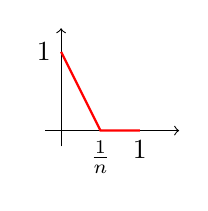
\begin{tikzpicture}
				\draw[->] (-0.2,0) -- (1.5,0);
				\draw[->] (0,-0.2) -- (0,1.3);

				\draw[red, thick] (0,1) node [black, left] {1} -- (0.5,0) node [black, below] {$\frac{1}{n}$} -- (1,0) node [black, below] {$1$};
			\end{tikzpicture}
			\caption{}
			\label{fig:ejemploContinuidadPuntual}
			\end{figure}

			\[
			\lim_{n \rightarrow \infty} f_n(x) = \begin{cases}
			1 & x = 0\\
			0 & x \neq 0
			\end{cases} \quad \text{ lo cual no es contínuo }
			\]

			Ojo, la función en \ref{fig:ejemploContinuidadPuntual1b} función es $c^{\infty}$, pero converge puntualmente a lo mismo.

			\begin{figure}[thbp]
			\centering
			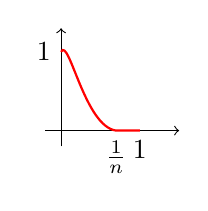
\begin{tikzpicture}
				\draw[->] (-0.2,0) -- (1.5,0);
				\draw[->] (0,-0.2) -- (0,1.3);

				\draw[red, thick] (0,1) node [black, left] {1} .. controls (0.1,1.2) and (0.3,0.05) .. (0.7,0) node [black, below] {$\frac{1}{n}$} -- (1,0) node [black, below] {$1$};
			\end{tikzpicture}
			\caption{}
			\label{fig:ejemploContinuidadPuntual1b}
			\end{figure}

		\end{example}

		\begin{example}{2 De integral}

			\begin{figure}[thbp]
			\centering
			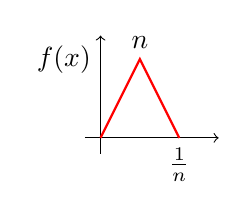
\begin{tikzpicture}
				\draw[->] (-0.2,0) -- (1.5,0);
				\draw[->] (0,-0.2) -- (0,1.3) node [below left] {$f(x)$};

				\draw[red, thick] (0,0) -- (0.5,1) node [black, above] {$n$} -- (1,0) node [black, below] {$\frac{1}{n}$};
			\end{tikzpicture}
			\caption{}
			\label{fig:ejemploContinuidadPuntual2}
			\end{figure}

		\[ \lim_{n \to \infty} fn(x) = 0 \quad \forall x \]

		\[ \int_0^1 f_n(x) dx = \frac{1}{2} \quad \forall n \]

		\[ \lim_{n \to \infty} \int_0^1 f_n(x) dx = \frac{1}{2} \neq \int_0^1 \lim_{n \to \infty} f_n(x)  dx = 0  \]


		\end{example}


	\subsubsection{Convergencia uniforme}

		\begin{defn}[Convergencia\IS uniforme]

			$\{f_n\}$ converge a $f$ uniformemente en $(a,b) \Leftrightarrow$ para todo $\epsilon > 0$, podemos encontrar ${n_0 = n_0(\epsilon)}$ tal que si $n \geq n_0$ entonces $|f_n(x) - f(x)| < \epsilon$, $\forall x \in (a,b)$.

			Lo que es equivalente a
			\[
				\sup_{x \in (a,b)} |f_n(x) - f(x)| < \epsilon
			\iff
				\left.||f_n - f||_{\infty}\right|_{(a,b)} < \epsilon
			\]

			\textbf{Interpretación geométrica}

			Tenemos una banda de tamaño $2\epsilon$ alrededor de toda la gráfica de f, y si $n \geq n_0$, {\bf toda} la gráfica de $f_n$ está dentro de dicha banda.

			\begin{figure}[thbp]
			\centering
			\inputtikz{ConvergenciaUniforme}
			\caption{Interpretación geométrica de la convergencia uniforme}
			\label{fig:CochesCarril}
			\end{figure}

		\end{defn}

		\begin{theorem}

			Supongamos que $f_n \rightarrow f$ uniformemente en $(a,b)$.

			\begin{itemize}
				\item $f_n$ continuas en $(a,b) \Rightarrow f$ continua en $(a,b)$

				\item $f_n$ integrables, $(a,b)$ acotado

				\[\int^{b}_{a} f(x) dx = \lim_{n \rightarrow \infty} \int^{b}_{a} f_n(x) dx \]
			\end{itemize}

			\obs La convergencia uniforme no preserva la derivabilidad

		\end{theorem}

		\begin{example}{Valor absoluto}

			$\{f_n\}$ funciones ``redondeadas'' que convergen a el valor absoluto. Ver figura \ref{fig:convergenciaValorAbsoluto}

			\begin{figure}[thbp]
			\centering
			\inputtikz{convergenciaValorAbsoluto}
			\caption{}
			\label{fig:convergenciaValorAbsoluto}
			\end{figure}

			\[f_n(x) = \sqrt{x^2 + 1/n} \convs[][n][\infty] \sqrt{x^2} = |x| \]

		\end{example}

	\subsubsection{Convergencia en $L^2$}

		\begin{defn}[Convergencia\IS en $L^2$]

			$L^2((a,b)) = \{$ funciones integrables en $(a,b)$ tales que $\int\limits_{a}^{b} |f(x)|^2 dx < \infty \}$

			En $L^2$ tenemos:
			\begin{itemize}
				\item Norma: $||f||_2 = \left( \int^{b}_{a} |f|^2 dx \right)^{\frac{1}{2}}$

				\item Producto escalar asociado: $<f,g> = \int\limits^b_a f(x) g(x) dx $

				\item $f_n \eqexpl[\rightarrow]{$L^2$} f \iffdef ||f_n - f||_2 \convs 0 $
			\end{itemize}

			Por lo que podemos entender $L^2$ como el cierre del conjunto de las funciones continuas en $(a,b)$ respecto a la norma 2 ($||\,||_2$).

			Entonces si $f \in L^2$, $\exists \{f_n\} \subset \{$ contínuas $\}$, tales que $f_n \eqexpl[\rightarrow]{$L^2$}f$.
		\end{defn}

		\begin{defn}[Convergencia\IS en $L^p$]

			\[L^p \rightarrow \|f\|_{p} = \left( \int^{b}_a |f|^p dx \right)^{\frac{1}{p}} \text{ para } 1 \leq p < \infty \]

		\end{defn}

			Y si vamos a $L^\infty$, lo que tenemos es la norma infinito, es decir, la norma supremo.

			\obs si $p\neq 2$, en $L^p$ no hay producto escalar, y las cuentas se complican.

			Podría ser interesante estudiar para qué valores de $p$ las series de Fourier convergen, pero esto se sale del alcance de esta asignatura.

	% clase 2016/02/17

	\subsubsection{Relaciones entre las convergencias}

		\begin{itemize}
			\item Convergencia uniforme $\Rightarrow$ Convergencia puntual.

			\item Convergencia uniforme en $(a,b)$, \textbf{acotado} $\Rightarrow$ Convergencia $L^2$
			\begin{proof}
				\[f_n \rightarrow f \text{ uniforme en } (a,b) \]
				\[ \left( \int^{b}_a |fn-f|^2 dx \right)^{\frac{1}{2}} \eqexpl[<]{$n > n_0$} \left( \int^{b}_a \epsilon^2 dx \right)^{\frac{1}{2}} = \epsilon \sqrt{b-a} \rightarrow 0 \]
			\end{proof}

				\begin{obs}
					Esto es falso en general en conjuntos no acotados (DIBUJOS EXPLICACIÓN)

					Esto está relacionado con el hecho de que si (a,b) no acotado entonces límite e integral no permutan.
				\end{obs}

			\item Convergencia $L^2 \not \Rightarrow $ convergencia uniforme

				\begin{example}
					Usando el mismo ejemplo que en la figura \ref{fig:ejemploContinuidadPuntual}

					\[ 0 \leq \int^1_0 |f_n|^2 dx \eqreason[\leq]{$0 \leq f_n \leq 1 \Rightarrow 0 \leq f_n^2 \leq f_n$} \int^1_0 |f_n| dx \eqreasonup{Área triángulo} \frac{1}{2n} \convs[ ][n][0] \infty \]

					De esto se deduce que:

					\[f_n \eqexpl[\rightarrow]{$L^2$} 0\]
					\[f_n \not \rightarrow 0 \text{ uniformemente, ya que } \lim f_n =
					\begin{cases}
						1 & x = 0\\
						0 & x \neq 0
					\end{cases}\]
				\end{example}

			\item Convergencia en $L^2 \not \Rightarrow $ convergencia puntual

				\begin{example}
					\[g_n = (-1)^n f_n \text{ (ejemplo anterior)}\]
					\[g_n \eqexpl[\rightarrow]{$L^2$} 0 \ \text{ , pero  } \ g_n(0) = (-1)^n \text{ que no converge.}\]

				\end{example}

			\item Convergencia puntual $\not \Rightarrow $ convergencia en $L^2$

				\begin{example}

					Utilizamos el mismo ejemplo visto en la figura \ref{fig:ejemploContinuidadPuntual2}.

					\[h_n^2 \convs 0 \text{ puntualmente, pero } \int_0^1 |h_n|^2 dx = \frac{1}{2} \forall n \]
				\end{example}

		\end{itemize}

		De estas implicaciones y no implicaciones obtenemos los diagramas \ref{fig:diagramaConvergenciasAcotado} y \ref{fig:diagramaConvergenciasNoAcotado}.

		\begin{figure}[thbp]
		\centering
		\inputtikz{diagramaConvergenciasAcotado}
		\caption{Implicaciones para un dominio acotado}
		\label{fig:diagramaConvergenciasAcotado}
		\end{figure}

		\begin{figure}[thbp]
		\centering
		\inputtikz{diagramaConvergenciasNoAcotado}
		\caption{Implicaciones para un dominio no acotado}
		\label{fig:diagramaConvergenciasNoAcotado}
		\end{figure}

	\subsubsection*{Problema}

		Dar sentido a una expresión de la forma:

		\[ f(x) = \frac{a_0}{2}+ \sum_k a_k \cos \left( \frac{k \pi}{L} x \right) + \sum_k b_k \sin \left( \frac{k \pi}{L} x \right) \]

		\textbf{Interpretación:}

		\[
		\{\frac{a_0}{2},a_k,b_k\}_{k=1,2,…} \equiv \text{ ``Coordenadas'' de f respecto}\]
		\[\text{ respecto de la ``base'' } \{1, \cos \left( \frac{k \pi}{L} x \right), \sin \left( \frac{k \pi}{L} x \right) \}_{k \in \nat }\]

		\obs Las comillas las ponemos porque estamos hablando de un EV con infinitas dimensiones.

		\begin{theorem}[Condiciones de ortogonalidad] $ $ % hack para que el primer item no se "suba" hasta el título

			\begin{enumerate}[label=(\arabic*)]

				\item
				\[ \int^{L}_{-L} \cos \left( \frac{k \pi}{L} x \right) dx = \int^{L}_{-L} \sin \left( \frac{k \pi}{L} x \right) dx = 0, \forall k \]

				\[\Rightarrow <\cos \left( \frac{k \pi}{L} x \right),1>_{L^2} = < \sin \cos \left( \frac{k \pi}{L} x \right),1>_{L_2} = 0\]

				\item
				\[ \int^{L}_{-L} \cos \left( \frac{k \pi}{L} x \right) \cdot \sin \left( \frac{j \pi}{L} x \right) dx = 0, \forall k, \forall j\]

				\[\Rightarrow < \cos \left( \frac{k \pi}{L} x \right), \sin \left( \frac{j \pi}{L} x \right) >_{L_2} = 0   \]

				\item
				\[ \int^{L}_{-L} \cos \left( \frac{k \pi}{L} x \right) \cdot \cos \left( \frac{j \pi}{L} x \right) dx = \begin{cases}
				0 & k \neq j \\
				L & k = j \end{cases} \]

				\[ \int^{L}_{-L} \sin \left( \frac{k \pi}{L} x \right) \cdot \sin \left( \frac{j \pi}{L} x \right) dx = \begin{cases}
				0 & k \neq j \\
				L & k = j \end{cases} \]

				\[\Rightarrow < \cos \left( \frac{k \pi}{L} x \right), \cos \left( \frac{j \pi}{L} x \right) >_{L_2} = \begin{cases}
				0 & k \neq j \\
				L & k = j \end{cases} \]

				\[ < \sin \left( \frac{k \pi}{L} x \right), \sin \left( \frac{j \pi}{L} x \right) >_{L_2} = \begin{cases}
				0 & k \neq j \\
				L & k = j \end{cases} \]

			\end{enumerate}
		\end{theorem}

			\begin{proof}

				\begin{itemize}
					\item Usar fórmulas trigonométricas

						\[\cos(A ± B), \sin(A ± B), …\]

					\item Usar complejos:

						\[ \cos(\theta) = \frac{e^{i\theta} + e^{-i\theta} }{2}, \quad \sin(\theta) = \frac{e^{i\theta} - e^{-i\theta} }{2i}\]

						\[  \int^{L}_{-L} \cos \left( \frac{k \pi}{L} x \right) \cdot \sin \left( \frac{j \pi}{L} x \right) dx = \]

						\[ = \int^L_{-L} \frac{e^{i\frac{k\pi}{L}x} + e^{-i\frac{k\pi}{L}x} }{2} \cdot \frac{e^{i\frac{j\pi}{L}x} - e^{-i\frac{j\pi}{L}x} }{2i} dx = … = 0 \]

				\end{itemize}

			\end{proof}


		% Aquí no he incluido una observación sobre un ejercicio en particular de la hoja


	\subsubsection{Cálculo de los coeficientes}

		La idea es que cada coeficiente es la proyección de f en una dirección, de las infinitas direcciones que nos da la base.

		\textbf{Idea:} fijémonos en el caso de la suma finita

		\[ f(x) = \frac{a_0}{2}+ \sum_{k=1}^M a_k \cos \left( \frac{k \pi}{L} x \right) + \sum_{k=1}^M \sin \left( \frac{k \pi}{L} x \right)\]

		Ahora fijamos $k=k_0$:

		\[ \int^L_{-L} f(x) \cos \left( \frac{k_0 \pi}{L} x \right) dx = \int^L_{-L} (\frac{a_0}{2} + \sum_k + \sum_k ) \cdot  \cos \left( \frac{k \pi}{L} x \right) dx  = \]

		\[ \frac{a_0}{2}  \int^L_{-L} \cos \left( \frac{k_0 \pi}{L} x \right) dx +\\
		\sum_k^M a_k \int^L_{-L} \cos \left( \frac{k_0 \pi}{L} x \right) \cos \left( \frac{k \pi}{L} x \right) dx +
		\sum_k^M b_k \int^L_{-L} \sin \left( \frac{k_0 \pi}{L} x \right) \sin \left( \frac{k \pi}{L} x \right) dx \]

		Hemos cambiado de orden el sumatorio y la integral. En el caso de sumas finitas podemos hacerlo porque la integral es un operador lineal, pero debemos justificarlo para el caso de sumas infinitas.

		Volviendo a la cuenta que tenemos entre manos, tenemos que todas las integrales que estamos sumando son 0 menos una:

		\[ \dots = a_{k_0} \cdot L \rightarrow a_{k_0} = \frac{1}{L} \int^{L}_{-L} f(x) \cos \left( \frac{k_0 \pi}{L} x \right) dx \]

		Análogamente:
		\[ b_{k_0} = \frac{1}{L} \int^L_{-L} f(x) \sin \left( \frac{k_0 \pi}{L} x \right) dx \]

		Quedaría por comprobar que $$a_0 = \frac{1}{L} \int^L_{-L} f(x) dx $$

		Pero tenemos un problema para justificar el cálculo cuando $M \rightarrow \infty$: permutar integral y suma infinita \[ \int \sum_1^{\infty} \qeq \sum_1^{\infty} \int\]

		Podemos definir:
		\[a_0 = \frac{1}{L} \int_{-L}^L f(x) dx \]
		\[a_k = \frac{1}{L} \int_{-L}^L \cos \left( \frac{k \pi}{L} x \right) dx  \]
		\[b_k = \frac{1}{L} \int_{-L}^L f(x) \sin \left( \frac{k \pi}{L} x \right) dx  \]

		\textbf{Idea:} Dada $f(x)$ podemos calcular $a_0, a_k, b_k$ y construir:

		\[ f(x) \eqreason[≈]{¿En qué casos podremos poner un $=$?} \frac{a_0}{2} + \sum_{k=1}^{\infty} a_k \cos \left( \frac{k \pi}{L} x \right) dx + \sum_{k=1}^{\infty} b_k \sin \left( \frac{k \pi}{L} x \right) dx \]


		Veamos en que puntos la serie de la derecha converge. Pero necesitamos ver también que converge a la $f(x)$ de la que habíamos partido. No es trivial y solo se cumplirá en algunos casos.

		¿Por qué ocurre esto? La definición de límite tiene una limitación, que es necesario saber el límite para escribirlo. Cuando no lo sabemos, podemos usar el criterio de Cauchy para demostrar convergencia y demostrar que existe el límite. Desgraciadamente Cauchy no nos dará el valor del límite.

		Veamos que herramienta vamos a utilizar para calcular este límite:

		\begin{defn}[Criterio\IS de Weierstrass]\label{defn:criterio_Weierstrass}

			Supongamos que tenemos $\{\Phi_k\}$ sucesión de funciones en $(a,b)$, tales que para cada $k$, existe $M_k \in \real$ con $|\Phi_k(x)| \leq M_k$, $\forall x \in (a,b)$.

			Entonces: Si $\sum\limits_{k=1}^{\infty} M_k < \infty$, la serie $\sum\limits_{k=1}^{\infty} \Phi_k(x) $ converge uniformemente en $(a,b)$.


			\begin{proof}
				Queremos demostrar que la sucesión $\{\sum\limits_{k=1}^{N} \Phi_k(x)\}_{N=1,2,…} $ converge uniformemente en $(a,b)$.

				Criterio de Cauchy:\index{Criterio!de Cauchy} Basta probar que $\forall \epsilon > 0, \exists n_0 $ tal que $n,m \geq n_o $, entonces:

				\[ | \sum^n_1 \Phi_k(x) - \sum^m_1 \Phi_k(x) | < \epsilon \quad \forall x \in (a,b) \]

				Suponiendo que $n > m$:
				\[| \sum^{N}_1 \Phi_k (x) - \sum^{m}_1 \Phi_k (x) | = | \sum^n_{k=m+1} \Phi_k | \leq \sum^n_{k=m+1} | \Phi_k (x) | \leq \sum_{m+1}^n m_k < \epsilon \]

				si $n,m$ son grandes por ser  $\sum\limits_{1}^{\infty} m_k < \infty $.

			\end{proof}
		\end{defn}

		\begin{example}{Ejercicio para el lector}

			\[ f \in C^2 ([-L,L]), 2L-\text{periódica}\]
			\[ a_k = \frac{1}{L} \int^{L}_{-L} f(x) \cos \left( \frac{k \pi}{L} x \right) dx \]

			Demostrar $|a_k| < \frac{C}{K^2}$

			(Análogamente $|b_k| < \frac{C}{k^2}$)

			Usando $\sum \frac{1}{k^2} < \infty$.
		\end{example}

		\obs Hasta ahora hemos demostrado que la suma converge a una función, pero no que converja a $f(x)$.

		Retomemos las fórmulas anteriores:

		\[ f(x) ≈ \frac{a_0}{2} + \sum_{k=1}^\infty a_k \cos \left( \frac{k \pi}{L} x \right) + \sum_{k=1}^\infty b_k \sin \left( \frac{k \pi}{L} x \right) \]

		\[a_k = \frac{1}{L} \int_{-l}^L \cos \left( \frac{k \pi}{L} s \right) f(s) ds \]

		\[ f \in C^2 ([-L,L]), f(-L) = f(L) \]

		\[a_k = \frac{1}{L} \int^L_{-L} \cos \left( \frac{k \pi}{L} s \right) f(s) ds \eqreasonup{partes} \frac{1}{L} \left\{ \left. f(s) \frac{\sin \left( \frac{k \pi}{L} s \right)}{\frac{k \pi}{L}} \right|_{s=-L}^{L} -  \int^L_{-L} f'(s) \frac{\sin \left( \frac{k \pi}{L} s \right)}{\frac{k \pi}{L}} ds   \right\}  \]

		\[ = \frac{1}{k\pi} -  \int^L_{-L} f'(s) \sin \left( \frac{k \pi}{L} s \right) ds \eqreasonup{partes} … \leq \frac{C}{k^2} \]

		Análogamente: $b_k \leq \frac{C}{k^2}$.

		% clase 2016/02/22

		\textbf{Conclusión:} criterio de Weierstrass $\Rightarrow$ convergencia uniforme en $[-L,L]$.

		\obs ojo, Si $f \in C^3$ (más condiciones de periodicidad) podría hacer partes otra vez y obtener la cota $\frac{C}{K^3}$. Y así hasta $C^n$: cuanta mayor regularidad le pidamos a la $f$ (y las condiciones de periodicidad oportunas para las cancelaciones) mayor orden tendrá el $\frac{1}{k}$.

		Veamos también que hay un problema sutil:

		\[f \rightarrow \text{ calculo } \{a_0,a_k,b_k\} \rightarrow \text{ construyo serie que converge } \]

		Pero esa serie, ¿converge a $f$?

		\begin{lemma}
			Supongamos $\sum \Phi_k$ converge uniformemente en $(a,b)$ y sea $h(x)$ contínua.

			\begin{itemize}
				\item $\sum_k h \Psi_k$ converge uniformemente en $(a,b)$ y además:
				\[ \sum_k h \Psi_k = h \sum \Psi_k\]

				\item \[\int_a^b \sum_k h \Psi_k = \sum_k \int_a^b h \Psi_k \]
			\end{itemize}

		\end{lemma}

		Este lema justifica que los coeficientes del desarrollo trigonométrico de$$g(x) = a_0 + \sum a_k \cos \left( \frac{k \pi}{L} x \right) + \sum b_k \sin \left( \frac{k \pi}{L} x \right) $$ son $\{a_0,a_k,b_k\}_{k \in \nat}$

		\textbf{Convergencia uniforme}

		$f \in C^2$, periódica $\Rightarrow$ la serie converge uniformemente.

		Problema: identificar el límite.

		Como $L^2$, nuestra base es: $\{1, \cos \left( \frac{k \pi}{L} x \right), \sin \left( \frac{k \pi}{L} x \right)\}_{k \in \nat}$

		\obs Si $f$ es discontinua en un punto, la integral ``no se entera'' y la transformación de Fourier me da la versión contínua de $f$.

		Tenemos que $\{1, \cos \left( \frac{k \pi}{L} x \right), \sin \left( \frac{k \pi}{L} x \right)\}_{k \in \nat}$ es ortogonal.

		Vamos a calcular los módulos para normalizar:

		\[\|1\|_{L^2 (-L,L)} = \left( \int_{-L}^L \cos^2  \left( \frac{k \pi}{L} s \right) ds \right)^{1/2} = \sqrt{2L} \]

		\[\left\|\cos \left( \frac{k \pi}{L} x \right)\right\|_{L^2 (-L,L)} = \left( \int_{-L}^L \cos^2  \left( \frac{k \pi}{L} s \right) ds \right)^{1/2} = \eqreason[…]{$\cos(2s) = \cos^2 \theta - \sin^2 \theta = 2\cos^2(\theta) - 1$}  = \sqrt{L} \]

		El del seno es similar y también tiene como resultado $\sqrt{L}$.

		Con lo que llegamos a la base ortonormal: $\{\frac{1}{\sqrt{2L}}, \frac{1}{\sqrt{L}} \cos \left( \frac{k \pi}{L} x \right),\frac{1}{\sqrt{L}} \sin \left( \frac{k \pi}{L} x \right)\}_{k \in \nat}$


		\[ f(x) ≈ \frac{a_0}{2} + \sum_{k=1}^\infty a_k \cos \left( \frac{k \pi}{L} x \right) + \sum_{k=1}^\infty b_k \sin \left( \frac{k \pi}{L} x \right) \]

		\[ a_k \cos \left( \frac{k \pi}{L} x \right) = \int^L_{-L} \frac{1}{L} \cos \left( \frac{k \pi}{L} s \right) ds \frac{1}{\sqrt{L}} \cos \left( \frac{k \pi}{L} x \right) = \]

		\[ = < f, \frac{1}{\sqrt{L}} \cos \left( \frac{k \pi}{L} s \right)> \cdot \frac{1}{\sqrt{L}} \cos \left( \frac{k \pi}{L} x \right) \]


		\textbf{Notación}

		$\{ \Phi_k \} $ sistema ortonormal en $L^2$, ($<\Phi_k,\Phi_j>_{L^2} = \delta_{kj}$).

		\[ f ≈ \sum_k < f, \Phi_k >_{L^2} \cdot \Phi_k (x) \]

		\textbf{Notación compleja}

		Usando $e^{i\theta} = \cos \theta + i \sin \theta$:

		\[
		\left. \begin{array}{r}
			a_k = \frac{1}{L} \int^{L}_{-L} \cos \left( \frac{k \pi}{L} s \right) f(s) ds\\
			b_k = \frac{1}{L} \int^{L}_{-L} \sin \left( \frac{k \pi}{L} s \right) f(s) ds
		\end{array} \right| \begin{array}{l}
			\frac{a_k - ib_k}{2} = \frac{1}{2L} \int_{-L}^L f(s) e^{-i \left( \frac{k \pi}{L} s \right)} ds \\
			\frac{a_k + ib_k}{2} = \frac{1}{2L} \int_{-L}^L f(s) e^{+i \left( \frac{k \pi}{L} s \right)} ds \\
		\end{array}
		\]

		y definimos:
		\[
			\alpha_k = \frac{a_k - ib_k}{2}, \quad \alpha_{-k} = \frac{a_k + ib_k}{2}
		\]

		Esto también da un sistema ortogonal, pero ¿cómo normalizamos?:

		\[\left\{ e^{i \left( \frac{k \pi}{L} s \right)} \right\}_{k = 0,±1,±2,…} \]

		Vamos a ver que pasa con $L^2$ y las funciones con variable compleja:

		\[<f,g>_{L^2} = \int^L_{-L} f(x) \conj{g(x)} dx \]

		Luego:

		\[ \alpha_k = \frac{1}{2L} \int^L_{-L} f(s) e^{-i \left( \frac{k \pi}{L} s \right)} ds = \frac{1}{2L} \int_{-L}^L f(s) \conj{e^{i \left( \frac{k \pi}{L} s \right)}} ds = \frac{1}{2L} <f, e^{i \left( \frac{k \pi}{L} x \right)}> \]

		Ahora normalizamos:
		\[
		\left\|e^{i \left( \frac{k \pi}{L} x \right)}\right\|_{L^2} = \left( < e^{i \left( \frac{k \pi}{L} x \right)}, e^{i \left( \frac{k \pi}{L} x \right)} >_{L^2} \right)^{\frac{1}{2}} = \left( \int^{L}_{-L} e^{i \left( \frac{k \pi}{L} x \right)} \cdot \conj{ e^{i \left( \frac{k \pi}{L} x \right)}} dx \right)^{\frac{1}{2}} = \sqrt{2L}
		\]

		Con lo que llegamos al sistema ortonormal:

		\[
			\left\{ \frac{1}{\sqrt{2L}} e^{i \left( \frac{k \pi}{L} x \right)} \right\}_{k = 0, ±1, ±2, …}
		\]

		\[
		f ≈ \sum_{k=-\infty}^\infty \alpha_k e^{i \left( \frac{k \pi}{L} x \right)} = \sum_{k = -\infty}^\infty < f, \frac{1}{\sqrt{2L}} e^{i \left( \frac{k \pi}{L} x \right)} > = \frac{e^{i \left( \frac{k \pi}{L} x \right)}}{\sqrt{2L}}
		\]

		\obs Hay que diferenciar cuando hacemos producto escalar real del complejo.

		\textbf{Escribiremos:}

		\[ f ≈ \sum_k <f, \Phi_k> \cdot \Phi_k \]

		ya normalizado. $\|\Phi_k\|_2 = 1 \quad \forall k$.

		Definimos las sumas parciales (y luego estudiaremos el paso al límite):

		\[
		S_n f = \sum_{|k| < n} <f, \Phi_k> \Phi_k \begin{cases}
			\text{ en } \cplex & -n \leq k \leq n \\
			\text{ en } \real & 1 \leq k \leq n
		\end{cases}
		\]

		\[ \text{¿} \| f - S_n f \|_{L^2} \rightarrow 0 \text{?}\]

		Hagamos cuentas:

		\begin{itemize}

			\item
			\[ \|S_n f\|_{L^2}^2 = < S_n f, S_n f>_{L^2} = \sum_{|k| < n} <f, \Phi_k> \Phi_k \cdot \sum_{|j| < n} <f, \Phi_j> \Phi_j \]

			\[ \eqreason{$\sum$ finitas} \sum_{k,j} <f, \Phi_k><f, \phi_j>\underbrace{<\Phi_k, \Phi_j>}_{\delta_{kj}} = \sum_k | <f, \Phi_k> |^2
			\]

			Luego concluimos que $\|S_n f\|_{L^2}^2$ es creciente.

			\item
			\[
				<f, S_n f> = <f, \sum_{|k| < n} <f, \Phi_k> \Phi_k > \eqreason{$\sum$ finita} \sum_{|k| < n} | <f, \Phi_k> |^2
			\]

			\item
			\[
				0 \leq \|f - S_n f\|^2_{L} = <f - S_n f, f- S_n f> = <f,f> - 2 <S_n f, f> + <S_n f, S_n f>
			\]
			\[ = \|f\|_{L}^2 - \sum_{|k| < n} |<f, \Phi_k>|^2 \Rightarrow \sum_{|k| < N} |<f, \Phi_k>|^2 \leq \|f\|_L^2 \]

			\obs ¡Cuidado! en $\cplex: \ <S_n f, f> \neq < f, S_n f>$, hay que usar la siguiente propiedad:
			$$<f,g> = \gor{<g,f>} $$
		\end{itemize}

		\obs  \[
			\left.
			\begin{array}{l}
				\|S_n f\|^2_2 \text{ creciente } \\
				\|S_n f\|_2 \text{ acotado superiormente }
			\end{array}
			\right\} \Rightarrow \|S_n f\|_{2} \text{ converge }
		\]

		Pero ¿$\|S_n f\|_2 \convs \| f \|_2$?. Estamos en el mismo punto.

		\textbf{Conclusión:} Si demostramos que  $\|S_n f\|_{L^2} \rightarrow \| f \|_{L^2}$ entonces el último cálculo probaría que $S_n f \eqexpl[\rightarrow]{$L^2$} f$

		\obs De lo obtenido en el último cálculo tenemos que:

			\[ \sum_{|k| < n} |<f, \Phi_k>|^2 \leq \|f\|_2^2 \quad \forall n \]

			Haciendo tender a $n$ a $\infty$ obtenemos la \concept{Desigualdad\IS de Bessel}:

			\( \sum_{k=-\infty}^\infty |<f, \Phi_k>|^2 \leq \|f\|_2^2 \label{eq:desigualdad_bessel}  \)

			\obs En $\real^3$, esto equivale al teorema de Pitágoras, pero nos falta ver el $\geq$.

		% clase 2016/02/23
		\subsubsection{Cálculos en $\cplex$}
			De manera rápida, vamos a resumir los cálculos anteriores en $\cplex$, que aunque son parecidos, difieren en detalles.

			Comencemos definiendo las sumas parciales:
			$$S_n f = \sum\limits_{\abs{k}<n} <f, \Phi_k>\Phi_k$$
			Primero, calculemos el cuadrado de su norma:
			\begin{gather*}
			\|S_n f\|^2 = <S_n f, S_n f> = \int_{-L}^{L} \sum\limits_{\abs{k}<n} <f, \Phi_k>\Phi_k \cdot \gor{\sum\limits_{\abs{j}<n} <f, \Phi_j>\Phi_j} \ ds \eqreasonup{agrupar sumas y suma finita conmuta con integral}\\
			= \sum\limits_{\abs{k},\abs{j}<n} <f, \Phi_k> \gor{<f, \Phi_j>} \int_{-L}^{L} \underbrace{\Phi_k \gor{\Phi_j}}_{<\Phi_k, \Phi_j>} \ ds \eqreasonup{$<\Phi_k, \Phi_j> = \delta_{kj}$} \sum\limits_{\abs{k}<n} <f, \Phi_k> \gor{<f, \Phi_k>} \eqreasonup{def norma en $\cplex$} \\
			= \sum\limits_{\abs{k}<n} \| <f, \Phi_k> \|^2
			\end{gather*}

			Ahora vemos si la distancia a $f$ está acotada:
			$$0 \leq \| f - S_n f\|_2^2 = \|f\|^2 - \sum\limits_{\abs{k}<n} \| <f, \Phi_k> \|^2$$
			Lo cual implica que
			$$\sum\limits_{\abs{k}<n} \| <f, \Phi_k> \|^2 \leq \|f\|^2 \ \forall n \convs \sum\limits_{k=-\infty}^{k=\infty} \| <f, \Phi_k> \|^2 \eqreasonup[\leq]{Bessel} \|f\|^2 \eqreasonup[<]{$f \in L^2$} \infty$$

			{\bf Conclusión:}
			Si $f \in L^2$, entonces la norma del producto escalar de f por los elementos de la base $\Phi_k$ tiende a 0.

			Por lo que podemos introducir una versión del lema de Riemann-Lebesgue:

			\begin{lemma}{Riemman-Lebesgue}

				\[ f \in L^2 \Rightarrow |<f, \Phi_k>| \convs[ ][k][\infty] 0\]

			\end{lemma}

			Y damos un pequeño ejemplo de su aplicación:
			\begin{example}
				$$ \int_{-L}^{L} f(s) \cdot \cos(\frac{k\pi}{L}s) ds \convs[ ][k][\infty] 0$$
			\end{example}

	\subsection{Resumen}

		\subsubsection*{Convergencia uniforme}

			\begin{itemize}
				\item Sistema trigonométrico (o exponencial complejo).
				\item $f \in C^2$ periódica
				\item No identificamos el límite
				\item Los coeficientes decaen en función de la regularidad de f
			\end{itemize}

		\subsubsection*{Convergencia $L^2$}

			\begin{itemize}
				\item Resultados válidos para cualquier sistema ortonormal $\{ \Phi_x \}$
				\item $f \in L^2$
				\item No identificamos el límite
				\[\text{falta probar }\|S_N f\|_2 \convs \lim_{N \to \infty} \|f\|_2\]
				\item Hay que utilizar la Desigualdad de Bessel y el Lema de Riemman-Lebesgue

			\end{itemize}

		Tenemos un problema con estas convergencias en cuanto a que ninguna nos permite identificar el límite. Vamos a dar un pequeño rodeo para llegar a demostrar lo que queremos.

		Comencemos con un ejemplo, planteando otro \textbf{problema distinto:}
		\[
			\begin{cases}
				u_{xx} + u_{yy} = 0 & \text{ en } x^2 + y^2 < 1\\
				u(x,y) = f(x,y) & \text{ en } x^2 + y^2 = 1
			\end{cases}
		\]
		Con f tan regular como necesitemos.

		Hacemos el cambio a coordenadas polares:
		\begin{align*}
		 r^2 = x^2 + y^2  &\rightarrow rr_x = x , \quad r_x = \frac{x}{r} \eqreasonup{$x = r \cos \theta $} \cos \theta \\
		 \tan \theta = \frac{y}{x}  &\rightarrow \frac{1}{\cos^2 \theta} \theta_x = \frac{-y}{x^2}, \quad \theta_x = \frac{-y \cos^2\theta}{x^2} \eqreason{$y = r \sin \theta, x = r \cos \theta$} \frac{-r \sin \theta \cos^2 \theta}{r^2 \cos^2 \theta} = \frac{- \sin \theta}{r}
		\end{align*}
		Tenemos:
		\begin{align*}
			W(r, \theta) &= u(r \cos \theta, r \sin \theta)\\
			u_x &= W_r \cdot r_x + W_\theta \cdot \theta_x
		\end{align*}
		Sustituyendo $r_x$ y $\theta_x$ en $u_x$:
		\begin{align*}
			u_x = W_r \cdot \cos \theta + W_\theta \cdot \frac{- \sin \theta}{r}
		\end{align*}
		Ahora podemos calcular $u_{xx}$:
		$$ u_{xx} = (W_r \cdot \cos \theta + W_\theta \cdot \frac{- \sin \theta}{r})_x \ r_x + (W_r \cdot \cos \theta + W_\theta \cdot \frac{- \sin \theta}{r})_\theta \ \theta_x$$

		Se deja como ejercicio para el lector el resto de cuentas y repetir el procedimiento para obtener $u_y$ y $u_{yy}$. Al final obtenemos:
		$$ u_{xx} + u_{yy} = 0 = \dots = W_{rr} + \frac{1}{r}W_r + \frac{1}{r^2}W_{\theta\theta}$$
		Con \textbf{dato}:
		\[ u(x,y) = f(x,y), \text{ si } x^2 + y^2 = 1\]
		Luego
		\[ \underbrace{u(1 \cdot \cos \theta,1 \cdot \sin \theta)}_{W(1,\theta)} = f(\cos \theta, \sin \theta) \equiv g(\theta)\]

		Queremos resolver:
		\[
			\begin{cases}
			W_{rr} + \frac{1}{r} W_r + \frac{1}{r^2} W_{\theta \theta} = 0 & 0 < r < 1 \\
			W(1, \theta) = g(\theta) & \theta \in (-\pi,\pi)
			\end{cases}
		\]

		\begin{itemize}
			\item Necesitamos que $W$ sea continua en $r=0$
			\item $W$ es $2\pi$-periódica en $\theta$
		\end{itemize}

		Usamos el método de separación de variables, es decir, buscamos $$W(r, \theta) = R(r)\cdot \Phi(\theta)$$
		Vamos a sustituir en el sistema:
		\[R''\Phi + \frac{R'}{r}\Phi + \frac{R}{r^2} \Phi'' = 0 \]
		Y operamos
		\[ - \left( R'' \Phi + \frac{R'}{r}\Phi \right) = \frac{R}{r^2} \Phi'' \Rightarrow \underbrace{\frac{(r^2R''+rR')}{R}}_{\text{Función de }r} = \underbrace{\frac{\Phi''}{\Phi}}_{\text{Función de }\theta} = \lambda \in \real \]

		Luego necesitamos que
		\begin{itemize}
			\item $R$ continua en 0
			\item $\Phi$ $2\pi$-periódica
		\end{itemize}


		EDO en $\Phi$ (Ecuación de ondas)
		\[
			\begin{cases}
				\Phi'' = \lambda \Phi & \theta \in (-\pi, \pi) \\
				\Phi & 2\pi \text{ periódica }
			\end{cases}
		\]

		Como esta es la ecuación de ondas \ref{ec:ondas}, podemos plantar la solución:
		\[
			\begin{cases}
				\lambda_0 = 0,& \Phi_0 = c \in \real\\
				\lambda_k = -(\frac{\pi k}{L})^2 \eqreason{$\pi=L$} -k^2, & \Phi_k = A_k \cos (k\theta) + B_k \sin (k\theta)\\
				\lambda_k > 0 & \text{NO hay solución}
			\end{cases}
		\]

		Volvemos a la EDO en $r$ para ver sus soluciones a partir de las de $\Phi$:
		\begin{align*}
			\lambda_0 = 0 \implies & r\cdot R_0'' + R'_0 = 0\\
			& r\cdot R_0'' = - R'_0\\
			& \frac{R''_0}{R'_0} = \frac{-1}{r} \text{ (integramos) }\\
			& \ln(R'_0) = - \ln(r) + C \text{ (exponenciamos) }\\
			& R'_0 = \frac{A}{r}, \quad A \in \real \text{ (integramos) }\\
			& R_0 = A \cdot \ln(r) + B, \quad A,B \in \real
		\end{align*}
		Como $R_0(r)$ debe estar acotada y continua en 0, tenemos que $A = 0$, luego $$W_{0}(r, \theta) = A_0$$

		Vamos a ver qué ocurre con $\lambda_k = -k^2$:

		\[r^2 R''_k + r R'_k - k^2 R_k = 0 \quad \text{\bf Ecuación de Euler}\]\index{Ecuación! de Euler}
		Recordemos cómo se resuelve: buscamos soluciones de la forma
		\begin{align*}
			R_k &= r^\alpha \\
			R'_k &= \alpha r^(\alpha - 1) \\
			R''_k &= \alpha(\alpha-1)r^(\alpha - 2)
		\end{align*}
		Sustituimos en la ecuación original:
		\[ 0 = r^\alpha [\alpha(\alpha -1)+ \alpha - k^2] = r^\alpha [\alpha^2 - k^2] \]
		Y obtenemos que las raíces del polinomio característico son $\alpha = ± k$.

		Luego la solución quedaría:
		\[ R_k(r) = \alpha_k r^k + \beta_k r^{-k} \]
		Donde $\beta_k r^{-k}$ tiende a 0 porque buscamos soluciones continuas, luego acotadas.

		Finalmente, obtenemos que
		$$W_k(r, \theta) = r^k (A_k \cos(k\cdot \theta) + B_k \sin(k\cdot \theta))$$

		Luego nuestro {\bf candidato a solución}:
		\[\frac{A_0}{2} + \sum_{k=1} r^k \{A_k \cos(k \theta) + B_k \sin(k\theta)\}   \]

		Dato: $W(1,\theta) = g(\theta)$.

		Observamos que esta solución es buena porque si $r<1$, por el criterio de Weierstrass (\ref{defn:criterio_Weierstrass}), converge uniformemente en $[-\pi, \pi]$.

		Necesitamos:
		\[ g(\theta) \qeq \frac{x_0}{2} + \sum_{k = 1}^{\infty} A_k \cos(k \theta) + B_k \sin(k \theta) \]

		Debe ser entonces:

		\[
		\begin{array}{l}
			A_0 = \frac{1}{\pi} \int_{-\pi}^{\pi} g(s) ds \\
			A_k = \frac{1}{\pi} \int_{-\pi}^{\pi} g(s)\cos(ks) ds \\
			B_k = \frac{1}{\pi} \int_{-\pi}^{\pi} g(s) \sin(ks) ds \\
		\end{array}
		\]

		\begin{obs}
			\[ |A_0|, |A_k|, |B_k| < \frac{1}{\pi} \int_{-\pi}^{\pi} |g(s)| ds \]

			No necesitamos propiedades de regularidad, nos basta con que $g$ sea integrable.
		\end{obs}

		Podemos definir:

		\( W(r,\theta) = \frac{A_0}{2} + \sum_k r^k(a_k \cos(k \theta) + B_k \sin(k\theta)) \label{eq:serieW} \)

		Pero llegados aquí, nos preguntamos:

		\begin{itemize}
			\item ¿$W$ es solución?
			\item ¿$W(1, \theta) = g(\theta)$
		\end{itemize}


		La suerte que tenemos es que es una serie geométrica en $\cplex$, que con $r<1$ no solo converge, sino que podemos escribir la solución.

		Pasamos a notación compleja:
		\begin{align*}
			\alpha_k &= \frac{1}{2\pi} \int_{-\pi}^{\pi} g(s) e^{-iks} ds \\
			\alpha_k &= \frac{A_k - iB_k}{2} \\
			\alpha_{-k} &= \frac{A_k + iB_k}{2}
		\end{align*}

		Podemos reescribir \eqref{eq:serieW} entonces como:

		\begin{align*}
		W(r, \theta) &= \alpha_0 + \sum_{k=1}^{\infty} r^k \left( \alpha_k e^{ik\theta} + \alpha_{-k} e^{-ik\theta} \right)\\
%
		&= \sum_{k=0}^{\infty} \alpha_k r^k e^{ik\theta} + \sum_{l=1}^{\infty} \alpha_{-l} r^l e^{-il\theta} \quad (\text{Cambio: } k = -l)\\
%
		&= \sum_{k=0}^{\infty} \alpha_k r^k e^{ik\theta} + \sum_{k=-\infty}^{-1} \alpha_{k} r^{\abs{k}} e^{ik\theta} = \sum_{k=-\infty}^{\infty} \alpha_{k} r^{\abs{k}} e^{ik\theta}\\
%
		&= \sum_{k=-\infty}^{\infty} \underbrace{\left( \frac{1}{2\pi} \int_{-\pi}^{\pi} g(s) e^{-iks} ds \right)}_{\leq \frac{1}{2\pi} \int_{-\pi}^{\pi} |g(s)| ds < C} r ^{|k|} \underbrace{e^{ik\theta}}_{|e^{ik\theta}| \leq 1}\\
		\end{align*}
		Donde hemos aplicado el criterio de Weierstrass \ref{defn:criterio_Weierstrass}.

		% Clase 2016/02/24
		Si $r < 1$, tenemos que $\sum_k Cr^{|k|} < \infty$, luego tenemos convergencia uniforme de la serie $\sum_{k=-\infty}^{\infty} \alpha_{k} r^{\abs{k}} e^{ik\theta}$ y podemos intercambiar límite e integral:

		Por tanto, nuestra última ecuación es igual a:
		\[ = \frac{1}{2\pi} \int_{-\pi}^{\pi} g(s) \sum_{k=-\infty}^{\infty} r^{|k|} e^{ik(\theta-s)} ds \]

		Como $$\sum\limits_{k=-\infty}^{\infty} = \sum\limits_{k=0}^{\infty} + \sum\limits_{-1}^{-\infty}$$

		Por lo que obtenemos:

		\[
		\sum_{k=0}^{\infty} (\underbrace{r e^{i (\theta-s)}}_{|re^{i(\theta-s)}| < r < 1})^k \eqreasonup{\text{serie geométrica}} \frac{1}{1-re^{i(\theta-s)}}
		\]

		Realizamos el mismo proceso con la otra suma:
		\begin{gather*}
			\sum\limits_{-1}^{-\infty} r^{\abs{k}} e^{ik(\theta-s)} = \sum\limits_{-1}^{-\infty} r^{-k} e^{ik(\theta-s)} \eqreasonup{$k=-l$} \ \sum\limits_{1}^{\infty} r^{l} e^{-il(\theta-s)} = \sum\limits_{1}^{\infty} (r \cdot e^{-i(\theta-s)})^l = \frac{r \cdot e^{-i(\theta-s)}}{1-r \cdot e^{-i(\theta-s)}}
		\end{gather*}

		Y llegamos a la conclusión:
		\[
		W(r,\theta) = \frac{1}{2\pi} \int_{-\pi}^\pi g(s) \sum_{k=-\infty}^\infty r^{|k|} e^{ik(\theta-s)} = \frac{1}{2\pi} \int_{-\pi}^\pi g(s) \left\{ \frac{1}{1-re^{i(\theta-s)}} + \frac{re^{-i(\theta-s)}}{1-re^{-i(\theta-s)}} \right\} ds	\]

		Ahora usando números complejos, llegamos a la \concept{Integral\IS de Poisson de g}
		\[ = \int^{\pi}_{-\pi} g(s) \underbrace{\frac{1}{2\pi} \frac{1-r^2}{1+r^2-2r\cos (\theta - s)}}_{\text{\bf Núcleo de Poisson}} ds \]

		Ahora veremos la relación entre las propiedades de la serie y las propiedades del \concept{Núcleo\IS de Poisson}, que es:

		\[P(r,\alpha) = \frac{1}{2\pi} \frac{1-r^2}{1+r^2-2r\cos (\theta - s)} \]

		% revisado hasta acá

		\textbf{Propiedades}

		\begin{itemize}

			\item Fijo $r \in [0,1)$, $P(r,\alpha) = P(r,-\alpha)$, 2-$\pi$ periódico en $\alpha$.

			\item $P(r,\alpha) > 0$

			\item $\dpd{P}{\alpha} < 0$ en $\alpha \in [0,R)$

			\[ \text{En particular} \begin{cases}
				\max_{\alpha \in [\delta > 0, \pi)} P(r,\alpha) = P(r,\delta) \\
				\min P(r,\alpha) = P(r,\pi) = P(r,-\pi)
			\end{cases} \]

			\item \[
				\int_{-\pi}^\pi P(r, \alpha) d\alpha = 1 \quad \forall r < 1
			\]

			\begin{proof}
				Utilizar \[ \int_{-\pi}^\pi P(r, \alpha) = \frac{1}{2\pi} \int_{-\pi}^\pi \sum_{k=-\infty}^{\infty} r^{|k|} \cdot e^{ik\alpha}  = … = 1 + \frac{1}{2\pi}  \]
				(FALTA)
			\end{proof}


			\item \[
			\lim_{r \to 1^-} P(r, \alpha) = \begin{cases}
				\infty & \alpha = 0 \\
				0 & \alpha \neq 0
			\end{cases}
			\]

			\[
				\frac{1}{2\pi} \cdot \frac{1-r^2}{1+r^2-2r\cos \alpha} \rightarrow \begin{cases}
				\alpha = 0 & \frac{1}{2\pi} \frac{(1-r)(1+r)}{(1-r)^2} \rightarrow \infty \\
				\alpha \neq 0  & \frac{1}{2\pi} \frac{0}{\underbrace{2-2\cos \alpha}_{\neq 0}} = 0
				\end{cases}
			\]

			(DIBUJO ONDITAS ENTRE -pi y pi)

			Puesto que la función es periódica da lo mismo integrar entre $-\pi$ y $\pi$ que cualquier otro intervalo de tamaño $2\pi$. Todas serán 1.

			\begin{theorem}
				Supongamos que $g$ es una función contínua y $2\pi$-periódica. Entonces:

				\[ \int^\pi_{-\pi} g(s)P(r, \theta-s) ds \convs[][r][1^-] g(\theta) \text{ uniformemente en } [-\pi,\pi] \]

				IMPORTANTE: Este es el primer teorema que vemos en el que se nos indica el límite a parte de darnos convergencia uniforme. Usaremos este teorema como base para ampliar los resultados anteriores.

				\begin{proof}

					\[0 \leq \left| \int_{-\pi}^{\pi} g(s9 P(r, \theta-s) - g(\theta))  \right| \]

					Tenemos que $\int\limits_{-\pi}^{\pi} P(r, \theta-s) ds = 1$ por los cálculos anteriores, por lo que la multiplicaremos por lo que ya tenemos:

					\[0 \leq \left| \int_{-\pi}^{\pi} g(s9 P(r, \theta-s) - g(\theta))  \int\limits_{-\pi}^{\pi} P(r, \theta-s) ds  \right| \]

					\[ = \left| \int_{-\pi}^\pi (g(s) - g(\theta)) P(r, \theta - s) ds \right|  \leq \int^{\pi}_{-\pi} | g(s) - g(\theta) | P(r, \theta- s) \]

					Hemos podido hacer este paso ya que $P>0$, pero veremos en unos días que no se va a cumplir en otra prueba y tendremos problemas.


					(DIBUJO)

					Vamos a descomponer la integral en dos trozos, en uno nos ayudaremos de la continuidad de $g$ y en el otro de la del núcleo.

					\[ = \underbrace{\int_{|\theta-s|< \delta}}_{|g(s) - g(\theta)| \text{ pequeño y }p\text{ grande}} + \underbrace{\int_{|\theta-s| > \delta}}_{|g(s) - g(\theta)| \text{ acotado y }p\text{ pequeño}} \]

					Dado $\epsilon > 0$, $\exists \delta > 0$ tal que si $|\theta-s| < \delta$, entonces $|g(s) - g(\theta)| < \epsilon, \forall \theta$

					(FALTA UN POCO dos casos)

					Y volviendo a juntar tenemos:

					\[ \int^{\pi}_{-\pi} |g(s) - g(\theta) | \underbrace{P(r, \theta-s) ds}_{\leq P(r, \theta-(\theta-\delta)) = P(r, -\delta) = P(r, \delta)} \leq   \]

					\[\leq P(r, \delta) \int^{\pi}_{\theta+\delta} |g(s) - g(\theta) ds \leq C P(r, \underbrace{\delta}_{> 0}) \convs[][r][1^-] 0  \]

					\[g \text{ continua } \Rightarrow |g| < M \]

					\[ |g(s)  - g(\theta)| \leq |g(s)| + | g(\theta) | \leq 2m \]


					Hemos probado:

					Dado $\epsilon > 0$, $\exists r_0$ tal que si $r \in (r_0,1)$, (FALTA).

				\end{proof}

			\end{theorem}

			\textbf{Aplicación}

			\textbf{1:} $f$,$g$ continua, con los \textunderscore{los mismos} coeficientes de Fourier $\Rightarrow f \equiv g$

			\begin{proof}
				\[
					\left. \begin{array}{l}
					f \\
					g
					\end{array} \right\} \rightarrow \alpha_k \rightarrow \sum_k \alpha_k r^{|k|} e^{ek\theta} \left\{ \begin{array}{l}
						\int^{\pi}_{-\pi} f(s) P(r, \theta - s)ds \convs[][r][1^-] f \\
						\int^{\pi}_{-\pi} g(s) P(r, \theta - s)ds \convs[][r][1^-] g
					\end{array} \right.
				\]

				Por unicidad del límite $\Rightarrow f \equiv g$
			\end{proof}




		\end{itemize}

